\documentclass{article}
\usepackage[paper=a4paper,top=2cm,bottom=2cm,left=2cm,right=2cm]{geometry}
\usepackage{amsthm}
\usepackage{booktabs}
\usepackage{microtype}
\usepackage{siunitx}
\usepackage{tikz}
\usepackage{pxfonts}
\usepackage{hyperref}
\usepackage{cleveref}
\usepackage{makeidx}
\usepackage{framed}
\usepackage{etoolbox}
\usepackage{comment}
\usepackage{ucllcode}
\usepackage{bbding}
\usepackage{titlesec}

\ifdefined\fulledition
  \includecomment{extra}
  \specialcomment{example}{\vfill\begin{center}\begin{minipage}{.99\linewidth}\begin{framed}\begin{center}\begin{minipage}{.9\linewidth}\begin{center}\textsc{\bfseries Example}\end{center}}{\end{minipage}\end{center}\end{framed}\end{minipage}\end{center}\vfill}
\else
  \excludecomment{extra}
  \excludecomment{example}
\fi

\lstset{language=c++,basicstyle=\ttfamily,frame=lines,escapeinside=``}

\newcommand{\hex}[1]{\texttt{\bfseries #1}}

\titleformat{\section}[display]{\sc\bfseries\Large}{}{0.5ex}{\begin{minipage}{\textwidth}\rule{\textwidth}{1pt}\vspace{1mm}\begin{center}}[\end{center}\vspace{-0.5ex}\rule{\textwidth}{1pt}\end{minipage}]
\titleformat{\subsection}[display]{\sc\large\bfseries}{}{0ex}{\begin{minipage}{\textwidth}\begin{center}}[\end{center}\end{minipage}]

\begin{document}

\begin{extra}
\tableofcontents
\end{extra}

\clearpage

\section{Source Code Organisation}

\vfil
\code[title={foo.cpp}]{foo.cpp}
\vfil
\code[title={foo.h}]{foo.h}
\vfil

%%% Local Variables:
%%% mode: latex
%%% TeX-master: "full-edition.tex"
%%% End:

\section{Primitive Types}
\begin{center}
  \begin{tabular}{ll}
    \textbf{Type} & \textbf{Range} \\
    \toprule
    \tt char & -128 to 127 \\
    \tt short & -32768 to 32767 \\
    \tt int & -2147483648 to 2147483647 \\
    \tt long & -2147483648 to 2147483647 \\
    \tt long long & -9223372036854775808 to 9223372036854775807 \\
    \midrule
    \tt unsigned char & 0 to 255 \\
    \tt unsigned short & 0 to 65535 \\
    \tt unsigned int & 0 to 4294967295 \\
    \tt unsigned long & 0 to 4294967295 \\
    \tt unsigned long long & 0 to 18446744073709551615 \\
    \midrule
    \tt float & $1.17549 \times 10^{-38}$ to $3.40282 \times 10^{38}$ \\
    \tt double & $2.22507 \times 10^{-308}$ to $1.79769 \times 10^{308}$ \\
    \midrule
    \tt bool & {\tt true}, {\tt false} \\
    \bottomrule
  \end{tabular}
\end{center}
Ranges were determined using MSVC++2013 targetting Win64.
\begin{extra}
  \code[font size=\small,width=.95\textwidth]{primtypes.cpp}
\end{extra}


%%% Local Variables:
%%% mode: latex
%%% TeX-master: "full-edition"
%%% End:

\section{Pointers and References}

\subsection{Types}
\begin{center}
  \begin{tabular}{ll}
    Pointer to \verb'T' & \verb'T' \\
    Reference to \verb'T' & \verb'T&' \\
    Rvalue reference to \verb'T' & \verb'T&&' \\
    Unique pointer to \verb'T' & \verb'std::unique_ptr<T>' \\
    Shared pointer to \verb'T' & \verb'std::shared_ptr<T>' \\
  \end{tabular}
\end{center}

\subsection{Allocation}
\begin{center}
  \begin{tabular}{ll}
    Heap allocation (single object) & \tt new T({\it args}) \\
    Heap deallocation (single object) & \tt delete ptr \\
    Heap allocation (array) & \tt new T[{\it n}] \\
    Heap deallocation (array) & \tt delete[] ptr \\
    Unique pointer creation & \verb'std::make_unique<T>('{\it args}\verb')' \\
    Shared pointer creation & \verb'std::make_shared<T>('{\it args}\verb')' \\
    Moving unique pointer & \verb'std::move(ptr)' \\
  \end{tabular}
\end{center}


%%% Local Variables:
%%% mode: latex
%%% TeX-master: "full-edition"
%%% End:

\chapter{IO}

\begin{center}
  \begin{tabular}{ll}
    Header file & \verb'#include <iostream>' \\
    Standard input stream & \lstinline{std::cin} \\
    Standard output stream & \lstinline{std::cout} \\
    Reading from input stream & \lstinline{in >> var} \\
    Writing to output stream & \lstinline{out << var} \\
    Newline & \lstinline{std::endl} \\
  \end{tabular}
\end{center}

\begin{example}
  \code{hello-world.cpp}
\end{example}

\begin{example}
  \code{io-example.cpp}
\end{example}


%%% Local Variables:
%%% mode: latex
%%% TeX-master: "full-edition"
%%% End:

\chapter{Operators}

\begingroup
\newcommand{\overloadable}[2]{{\tt #1} & #2 & \Checkmark}
\newcommand{\notoverloadable}[2]{{\tt #1} & #2 & \XSolidBrush}

\begin{center}
  \begin{tabular}{c@{\hspace{1cm}}c}
    \begin{tabular}{llc}
      \rotatebox{45}{\textbf{Operator}} & \rotatebox{45}{\textbf{Description}} & \rotatebox{90}{\textbf{Overloadable}} \\
      \toprule
      \multicolumn{3}{c}{\bf\sc Unary prefix operators} \\
      \midrule
      \overloadable{+x}{} \\
      \overloadable{-x}{Negation} \\
      \overloadable{*x}{Dereferencing} \\
      \overloadable{!x}{Logical NOT} \\
      \overloadable{\&x}{Address of} \\
      \overloadable{\~{}x}{Bitwise NOT} \\
      \overloadable{++x}{Preincrement} \\
      \overloadable{--x}{Predecrement} \\
      \overloadable{new}{Allocation} \\
      \overloadable{delete}{Deallocation} \\
      \overloadable{sizeof}{Parameter pack} \\
      \midrule
      \multicolumn{3}{c}{\bf\sc Unary postfix operators} \\
      \midrule
      \overloadable{x++}{Postincrement} \\
      \overloadable{x--}{Postdecrement} \\
      \overloadable{x(...)}{Function call} \\
      \overloadable{x[y]}{Indexing} \\
      \notoverloadable{x.f}{Member access} \\
      \overloadable{x->f}{Member access} \\
      \bottomrule
    \end{tabular}
    &
    \begin{tabular}{llc}
      \rotatebox{45}{\textbf{Operator}} & \rotatebox{45}{\textbf{Description}} & \rotatebox{90}{\textbf{Overloadable}} \\
      \toprule
      \multicolumn{3}{c}{\bf\sc Binary infix operators} \\
      \midrule
      \overloadable{x + y}{Addition} \\
      \overloadable{x - y}{Subtraction} \\
      \overloadable{x * y}{Multiplication} \\
      \overloadable{x / y}{Division} \\
      \overloadable{x \% y}{Modulo} \\
      \overloadable{x \& y}{Bitwise AND} \\
      \overloadable{x | y}{Bitwise OR} \\
      \overloadable{x \^{} y}{Bitwise XOR} \\
      \overloadable{x \&\& y}{Logical AND} \\
      \overloadable{x || y}{Logical OR} \\
      \overloadable{x == y}{Equality} \\
      \overloadable{x != y}{Inequality} \\
      \overloadable{x < y}{Less than} \\
      \overloadable{x <= y}{Not greater than} \\
      \overloadable{x > y}{Greater than} \\
      \overloadable{x >= y}{Not less than} \\
      \overloadable{x, y}{Sequencing} \\
      \overloadable{x << y}{Shift left} \\
      \overloadable{x >> y}{Shift right} \\
      \bottomrule
    \end{tabular}
  \end{tabular}

    \begin{tabular}{llc}
      \rotatebox{45}{\textbf{Operator}} & \rotatebox{45}{\textbf{Description}} & \rotatebox{90}{\textbf{Overloadable}} \\
      \toprule
      \multicolumn{3}{c}{\bf\sc Binary infix operators} \\
      \midrule
      \overloadable{x += y}{Addition assignment} \\
      \overloadable{x -= y}{Subtraction assignment} \\
      \overloadable{x *= y}{Multiplication assignment} \\
      \overloadable{x /= y}{Division assignment} \\
      \overloadable{x \&= y}{Bitwise AND assignment} \\
      \overloadable{x |= y}{Bitwise OR assignment} \\
      \overloadable{x \^{}= y}{Bitwise XOR assignment} \\
      \overloadable{x <<= y}{Shift left assignment} \\
      \overloadable{x >>= y}{Shift right assignment} \\
      \bottomrule
    \end{tabular}
\end{center}

\endgroup

%%% Local Variables:
%%% mode: latex
%%% TeX-master: "full-edition"
%%% End:

\section{Flow Control}
Flow control statements are syntactically and semantically the same as in Java.

\subsection{Conditionals}
\vfil
\code{if-statement.cpp}
\vfil
\code[width=.5\linewidth]{switch-statement.cpp}
\vfil

\subsection{Iteration}
\code[width=.5\linewidth]{while-statement.cpp}
\code[width=.6\linewidth]{for-statement.cpp}
\code[width=.5\linewidth]{do-while-statement.cpp}


%%% Local Variables:
%%% mode: latex
%%% TeX-master: "full-edition"
%%% End:

\documentclass{ucll-slides}
\usepackage{ucll-code}
\usetikzlibrary{shadows,shapes.multipart}

\title{Casts}
\author{Fr\'ed\'eric Vogels}

\lstset{language=c++14}


\begin{document}

\begin{frame}
  \titlepage
\end{frame}

\begin{frame}
  \frametitle{Casting}
  \begin{itemize}
    \item Casting: explicit type conversion
    \item Upcasting: casting to a supertype
          \begin{itemize}
            \item E.g.\ cast from {\tt Dog} to {\tt Animal}
          \end{itemize}
    \item Downcasting: casting to a subtype
          \begin{itemize}
            \item E.g.\ cast from {\tt Animal} to {\tt Dog}
          \end{itemize}
    \item Upcasts are always safe
    \item Downcasts can go wrong
  \end{itemize}
  \code[font=\small,width=.9\linewidth]{wrong-downcast.cpp}
\end{frame}

\begin{frame}
  \frametitle{Casts in Java}
  \begin{itemize}
    \item Only one way to cast: {\tt (T) x}
    \item Java objects keep track of their ``real type'' (dynamic type)
    \item Casts are checked at runtime
    \item Wrong casts: {\tt IllegalCastException}
  \end{itemize}
\end{frame}

\begin{frame}
  \frametitle{Casts in \cpp}
  \begin{itemize}
    \item \cpp~has a few more casts
          \begin{itemize}
            \item C-style cast: {\tt (T) x}
            \item {\tt static\_cast<T>(x)}
            \item {\tt dynamic\_cast<T>(x)}
            \item {\tt reinterpret\_cast<T>(x)}
            \item {\tt const\_cast<T>(x)}
          \end{itemize}
          \vskip5mm
    \item Standard Library adds a few more
          \begin{itemize}
            \item {\tt std::static\_pointer\_cast<T>(x)}
            \item {\tt std::dynamic\_pointer\_cast<T>(x)}
          \end{itemize}
          \vskip5mm
    \item Most important for us: {\tt dynamic\_pointer\_cast<T>(x)}
  \end{itemize}
\end{frame}

\section{C-style casts}

\frame{\tableofcontents[currentsection]}

\begin{frame}
  \frametitle{C-style Casts}
  \structure{Syntax}
  \begin{center} \ttfamily
    (T) x
  \end{center}
  \vskip5mm
  \structure{Usage}
  \begin{itemize}
    \item Just don't use them
  \end{itemize}
\end{frame}

\section{Static and Dynamic Casts}

\frame{\tableofcontents[currentsection]}


\begin{frame}
  \frametitle{\texttt{static\_cast} and \texttt{dynamic\_cast}}
  \structure{\texttt{static\_cast<T>(x)}}
  \begin{itemize}
    \item Only checked at compile time
    \item Wrong casts lead to undefined results at runtime
  \end{itemize}
  \vskip5mm
  \structure{{\tt dynamic\_cast<T>(x)}}
  \begin{itemize}
    \item Checked at compile \emph{and} runtime
    \item Wrong casts give \texttt{nullptr}
    \item Is a bit slower due to runtime checks
    \item Only works on classes with 1+ virtual member functions
  \end{itemize}
\end{frame}

\begin{frame}
  \frametitle{Examples}
  \code[font=\small]{static-vs-dynamic-casts1.cpp}
\end{frame}

\begin{frame}
  \frametitle{Examples}
  \code[font=\small]{static-vs-dynamic-casts2.cpp}
\end{frame}

\begin{frame}
  \frametitle{Examples}
  \code[font=\small]{static-vs-dynamic-casts3.cpp}
\end{frame}

\begin{frame}
  \frametitle{Examples}
  \code[font=\small]{static-vs-dynamic-casts4.cpp}
\end{frame}

\begin{frame}
  \frametitle{Smart Pointers}
  \begin{itemize}
    \item We said not to use regular pointers {\tt T*}
    \item Use {\tt std::unique\_ptr} and {\tt std::shared\_ptr} instead
    \item Library offers specialised cast operators for {\tt std::shared\_ptr}
    \item \emph{No} specialised casts for {\tt std::unique\_ptr} (AFAICT)
  \end{itemize}
  \code[font=\small,width=.9\linewidth]{shared-ptr-casts.cpp}
\end{frame}

\section{{\tt reinterpret\_cast}}

\frame{\tableofcontents[currentsection]}


\begin{frame}
  \frametitle{{\tt reinterpret\_cast}}
  \begin{itemize}
    \item Anything goes
    \item No compile time checks
    \item No runtime checks
    \item Bad casts lead to undefined behaviour
  \end{itemize}
  \code[font=\small]{reinterpret_cast.cpp}
\end{frame}

\begin{frame}
  \frametitle{{\tt reinterpret\_cast}}
  \begin{itemize}
    \item Allows you to probe memory
    \item Breaks encapsulation
  \end{itemize}
  \begin{overprint}
    \onslide<handout:0|1>
    \code[font=\small]{find-password1.cpp}
    \onslide<handout:0|2>
    \code[font=\tiny,width=.9\linewidth]{find-password2.cpp}
    \onslide<handout:0|3>
    \code[font=\tiny,width=.8\linewidth]{find-password3.cpp}
  \end{overprint}
\end{frame}

{
  \newcommand{\HEX}[1]{\texttt{0x#1}}
  \newcommand{\fatentry}[3]{\HEX{#1} & #2 & #3 \\}

  \begin{frame}
    \frametitle{\texttt{reinterpret\_cast<T>(x)}: What's It Good For?}
    \begin{center} \Large
      Remember this?
    \end{center}
    \begin{center}
      \small
      \begin{tabular}{ccl}
        \textbf{Offset} & \textbf{Length} & \textbf{Description} \\
        \toprule
        \fatentry{00}{3}{Instructions to jump to the bootstrap code}
        \fatentry{03}{8}{Name of the formatting OS}
        \fatentry{0B}{2}{Bytes per sector}
        \fatentry{0D}{1}{Sectors per cluster}
        \fatentry{0E}{2}{Reserved sectors from the start of the volume}
        \fatentry{10}{1}{Number of FAT copies}
        \fatentry{11}{2}{Number of possible root entries}
        \fatentry{13}{2}{Small number of sectors}
        % \fatentry{15}{1}{Media descriptor}
        % \fatentry{16}{2}{Sectors per FAT}
        % \fatentry{18}{2}{Sectors per track}
        % \fatentry{1A}{2}{Number of heads}
        % \fatentry{1C}{4}{Hidden sectors}
        % \fatentry{20}{4}{Large number of sectors}
        % \fatentry{24}{1}{Drive number}
        % \fatentry{25}{1}{Reserved}
        % \fatentry{26}{1}{Extended boot signature}
        % \fatentry{27}{4}{Volume serial number}
        % \fatentry{2B}{11}{Volume label}
        % \fatentry{36}{8}{File system type --- should be \texttt{FAT12}}
        % \fatentry{3E}{448}{Bootstrap code}
        % \fatentry{1FE}{2}{Boot sector signature --- should be \HEX{AA55}}
        $\vdots$ & $\vdots$ & $\;\vdots$ \\
        \bottomrule
      \end{tabular}
    \end{center}
  \end{frame}
}

\begin{frame}
  \frametitle{FAT12}
  \code{fat12.cpp}
\end{frame}

\begin{frame}
  \frametitle{FAT12}
  \code[font=\small,width=\linewidth]{read-data.cpp}
\end{frame}

\begin{frame}
  \frametitle{{\tt reinterpret\_cast}}
   \begin{itemize}
    \item If you read raw bytes from
          \begin{itemize}
            \item Disk
            \item Network
            \item \dots
          \end{itemize}
    \item You can interpret raw data for what they represent
          \begin{itemize}
            \item FAT data tables
            \item IP address
            \item TCP/IP packets
            \item \dots
          \end{itemize}
  \end{itemize}
  \code[font=\small]{reinterpret.cpp}
\end{frame}

\section{{\tt const\_cast}}

\frame{\tableofcontents[currentsection]}

\begin{frame}
  \frametitle{{\tt const\_cast}}
  \begin{itemize}
    \item Used to remove {\tt const} qualified
    \item Only used for old C libraries
    \item Just don't use it
  \end{itemize}
  \code[font=\scriptsize,width=.95\linewidth]{const-cast.cpp}
\end{frame}

\end{document}


%%% Local Variables:
%%% mode: latex
%%% TeX-master: "casts"
%%% End:

\section{Classes}
\subsection{General syntax}
\code[width=.75\linewidth]{class.cpp}

\subsection{Inheritance}
\code[width=.75\linewidth]{inheritance.cpp}


%%% Local Variables:
%%% mode: latex
%%% TeX-master: "full-edition"
%%% End:

\documentclass{../ucll-slides}
\usepackage{../pvm}
\usetikzlibrary{shadows,shapes.multipart}

\title{Preprocessor}
\author{Fr\'ed\'eric Vogels}



\begin{document}

\begin{frame}
  \titlepage
\end{frame}

\begin{frame}
  \frametitle{Problem Statement}
  \begin{itemize}
    \item We've discussed forward declarations
    \item Forward declarations specify type information
    \item Compiler needs to keep this information in memory
    \item Large programs have large number of functions/classes
    \item Compiler can't fit all this data in memory
  \end{itemize}
\end{frame}

\begin{frame}
  \frametitle{Solution}
  \begin{itemize}
    \item Divide the codebase in small units
    \item ``Compilation units'' (CUs): {\tt .cpp} files
    \item In each file we put the minimal amount of declarations
    \item Compile each unit separately
    \item Link results together
  \end{itemize}
\end{frame}

\begin{frame}
  \frametitle{Build Steps}

  \begin{center}
    \begin{tikzpicture}[cpp/.style={draw,thick,drop shadow,fill=white,minimum width=2cm,minimum height=.75cm},
                        obj/.style={draw,thick,drop shadow,fill=white,minimum width=2cm,minimum height=.75cm},
                        exe/.style={draw,thick,drop shadow,fill=white,minimum width=2cm,minimum height=.75cm},
                        compile/.style={-latex,thick},
                        compile arc/.style={above,midway,font=\tiny},
                        link/.style={-latex,thick},
                        link arc/.style={above,midway,font=\tiny,sloped}]
      \node[cpp] (a cpp) at (0,4) {A.cpp};
      \node[cpp] (b cpp) at (0,2) {B.cpp};
      \node[cpp] (c cpp) at (0,0) {C.cpp};

      \visible<2->{
        \node[obj] (a obj) at (4,4) {A.obj};
      }

      \visible<2>{
        \draw[compile] (a cpp) -- (a obj) node[compile arc] {compile};
      }

      \visible<3->{
        \node[obj] (b obj) at (4,2) {B.obj};
      }

      \visible<3>{
        \draw[compile] (b cpp) -- (b obj) node[compile arc] {compile};
      }

      \visible<4->{
        \node[obj] (c obj) at (4,0) {C.obj};
      }

      \visible<4>{
        \draw[compile] (c cpp) -- (c obj) node[compile arc] {compile};
      }
      
      \visible<5->{
        \node[exe] (exe) at (8,2) {app.exe};
      }
      
      \visible<5>{
        \node[exe] (exe) at (8,2) {app.exe};
        \draw[link] (a obj) -- (exe) node[link arc] {link};
        \draw[link] (b obj) -- (exe) node[link arc] {link};
        \draw[link] (c obj) -- (exe) node[link arc] {link};
      }
    \end{tikzpicture}
  \end{center}
\end{frame}

\begin{frame}
  \frametitle{Example}
  \code[width=10cm,title={App.cpp},frame=lines]{ex1.cpp}
\end{frame}

\begin{frame}
  \frametitle{Example}
  \code[width=10cm,title={App.cpp},frame=lines]{ex1-decl.cpp}
\end{frame}

\begin{frame}
  \frametitle{Example}
  \code[width=10cm,title={foo.cpp},frame=lines]{ex1-foo.cpp}
  \code[width=10cm,title={bar.cpp},frame=lines]{ex1-bar.cpp}
  \code[width=10cm,title={qux.cpp},frame=lines]{ex1-qux.cpp}
\end{frame}

\begin{frame}
  \frametitle{Example}
  \begin{itemize}
    \item Each file can be compiled separately
    \item Each file contains minimal but sufficient declarations
  \end{itemize}
  \code[width=3cm]{decl.cpp}
  \begin{center}
    means \\[7mm]
    ``Some function {\tt foo} exists. It has one parameter of type {\tt int},
    and returns a {\tt bool}. If you do not encounter it in this file,
    I promise you you will find it in another one.''
  \end{center}
\end{frame}

\begin{frame}
  \frametitle{Linker}
  \begin{itemize}
    \item The compiler will believe your promises
    \item If you do not \emph{define} your declared function,
          compiler will assume it's in some other CU
    \item Linker is less naive
    \item Linker will check promises
    \item Missing \emph{definition} will lead to linker error
  \end{itemize}
\end{frame}

\begin{frame}
  \frametitle{Engineering Nightmare}
  \begin{center}
    \begin{tikzpicture}[definition/.style={fill=red!50,draw,rectangle split,rectangle split parts=2},
                        declaration/.style={fill=blue!50,draw,rectangle split,rectangle split parts=2},
                        reference/.style={-latex}]
      \node[definition] (definition) at (0,0) {
        def.cpp
        \nodepart{two}
        \tt void \only<1>{foo}\only<2->{{\color{red} bar}}() \{ \dots\ \}
      };

      \foreach[count=\i] \x in {0,60,...,300} {
        \node[declaration] (declaration \i) at (\x:3.5) {
          file\i.cpp
          \nodepart{two}
          \tikzmath{
            int \j;
            int \k;
            \j = int(\i + 1);
            \k = int(\j + 1);
          }
          \tt void \only<1-\j>{foo}\only<\k->{{\color{red}bar}}();
        };
        \draw[reference] (declaration \i) -- (definition);
      }
    \end{tikzpicture}
  \end{center}
\end{frame}

\begin{frame}
  \frametitle{Engineering Nightmare}
  \begin{itemize}
    \item Say the definition changes
          \begin{itemize}
            \item Name change
            \item Parameter change
            \item Return type change
          \end{itemize}
    \item Then all CUs containing a declaration need to be updated
    \item Due to redundancy: same declaration in many files
  \end{itemize}
\end{frame}

\begin{frame}
  \frametitle{Engineering Nightmare}
  \begin{itemize}
    \item Say the definition changes
          \begin{itemize}
            \item Name change
            \item Parameter change
            \item Return type change
          \end{itemize}
    \item Then all CUs containing a declaration need to be updated
    \item Due to redundancy: same declaration in many files
  \end{itemize}
\end{frame}

\begin{frame}
  \frametitle{Solution}
  \begin{itemize}
    \item Make {\tt cpp} file responsible for generating a list of declarations
          for all of its definitions
    \item Put these declarations in separate file
    \item Include the contents of this ``twin'' file in other {\tt cpp} files
    \item This ``twin'' file is called a \emph{header file}
  \end{itemize}
\end{frame}

\begin{frame}
  \frametitle{Header Files}
  \begin{columns}[t]
    \column{5cm}
    \code[width=5cm,title={funcs.cpp},frame=lines]{cpp-file.cpp}
    \column{5cm}
    \code[width=5cm,title={funcs.h},frame=lines]{header-file.h}
  \end{columns}
\end{frame}

\begin{frame}
  \frametitle{Including Header Files}
  \code[title={main.cpp},frame=lines,width=5cm]{including.cpp}
\end{frame}

\begin{frame}
  \frametitle{Visualisation}
  \begin{center}
    \begin{tikzpicture}[cpp/.style={fill=red!50,draw},
                        h/.style={fill=blue!50,draw},
                        includes/.style={-latex}]
      \foreach[count=\i] \x in {0,120,240} {
        \tikzmath{
          real \y;
          \y = \x + 90;
        }

        \node[cpp,rotate=\y] (file \i) at (\x:3) {
          file\i.cpp
        };

        \node[h,rotate=\y] (header \i) at (\x:2) {
          file\i.h
        };

        \draw[includes] (file \i) -- (header \i);
      }

      \draw[includes] (file 1) -- (header 2);
      \draw[includes] (file 2) -- (header 3);
      \draw[includes] (file 3) -- (header 1);

      \draw[includes] (file 1) -- (header 3);
      \draw[includes] (file 2) -- (header 1);
      \draw[includes] (file 3) -- (header 2);
    \end{tikzpicture}
  \end{center}
\end{frame}

\begin{frame}
  \frametitle{Typical Structure of {\tt cpp} file}
  \code[title={file.cpp},frame=lines]{header-example.cpp}
  \begin{itemize}
    \item First include: preferably own header file
    \item What's the reason for this? \cake
  \end{itemize}
\end{frame}

\begin{frame}
  \frametitle{Preprocessor}
  \begin{itemize}
    \item {\tt \#include} is a preprocessor directive
    \item Preprocessor is a separate minilanguage
    \item All code gets processed by the preprocessor first
  \end{itemize}
  \vskip4mm
  \begin{center}
    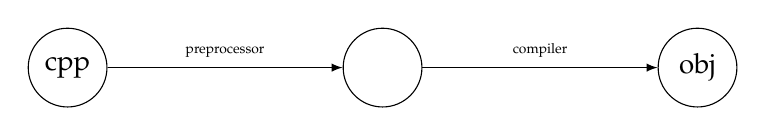
\begin{tikzpicture}[file/.style={circle,minimum size=1cm,draw},
                        translate/.style={-latex}]
      \node[file] (cpp) at (0,0) {cpp};
      \node[file] (intermediate) at (4,0) {};
      \node[file] (obj) at (8,0) {obj};

      \draw[translate] (cpp) -- (intermediate) node[midway,above,font=\tiny] {preprocessor};
      \draw[translate] (intermediate) -- (obj) node[midway,above,font=\tiny] {compiler};
    \end{tikzpicture}
  \end{center}
\end{frame}

\begin{frame}
  \frametitle{{\tt \#include Directive}}
  \begin{itemize}
    \item {\tt \#include "file"} is replaced by the contents of {\tt file}
    \item Works with \emph{any} file, on any line
    \item Preprocessor does not care about contents of files
  \end{itemize}
  \begin{columns}
    \column{5cm}
    \code[title={file.cpp},frame=lines,width=5cm]{include-example.cpp}
    \code[title={bla.txt},frame=lines,width=5cm]{bla.txt}
    \column{5cm}
    \code[title=result,frame=lines,width=5cm]{include-result.cpp}
  \end{columns}
\end{frame}

\begin{frame}
  \frametitle{Problem: Headers With Dependencies}
  \begin{center}
    \begin{tikzpicture}[file/.style={rectangle split,rectangle split parts=2,draw},
                        cpp/.style={file,fill=red!50},
                        h/.style={file,fill=blue!50},
                        includes/.style={-latex}]
      \node[cpp] (C cpp) at (0,0) {
        {\tt C.cpp}
        \nodepart{two}
        def.\ class {\tt C}
      };

      \node[h,anchor=north] (C h) at ($ (C cpp.south) + (0,-.5) $) {
        {\tt C.h}
        \nodepart{two}
        decl.\ class {\tt C}
      };

      \node[cpp] (foo cpp) at (4,0) {
        {\tt foo.cpp}
        \nodepart{two}
        void foo(C c) { \dots }
      };

      \node[h,anchor=north] (foo h) at ($ (foo cpp.south) + (0,-.5) $) {
        {\tt foo.h}
        \nodepart{two}
        void foo(C);
      };

      \node[cpp] (bar cpp) at (8,0) {
        {\tt bar.cpp}
        \nodepart{two}
        uses foo
      };

      \draw[includes] (C cpp) -- (C h);
      \draw[includes] (foo cpp) -- (foo h);
      \draw[includes] (foo cpp) -- (C h);
      \draw[includes] (bar cpp) -- (foo h);
    \end{tikzpicture}
  \end{center}
\end{frame}

\begin{frame}
  \frametitle{Problem: Headers With Dependencies}
  \begin{overprint}
    \onslide<1>
    \code[title=bar.cpp,frame=lines]{header-dependencies1.cpp}
    \onslide<2->
    \code[title=bar.cpp,frame=lines]{header-dependencies2.cpp}
  \end{overprint}
  \visible<3>{
    \begin{center}
      Compiler doesn't know type {\tt C}!
    \end{center}
  }
\end{frame}

\begin{frame}
  \frametitle{Proposed Solution \#1}
  \code[title=bar.cpp,frame=lines]{header-dependencies3.cpp}
  \begin{itemize}
    \item Have {\tt bar.cpp} also include {\tt C.h}
    \item Include order important $\rightarrow$ fragile
    \item Does {\tt bar.cpp} need to know of {\tt foo.h}'s dependency?
    \item If header file gets extra dependencies, all including {cpp} files
          would need to be updated
    \item Again, engineering nightmare
  \end{itemize}  
\end{frame}

\begin{frame}
  \frametitle{Proposed Solution \#2}
  \begin{overprint}
    \onslide<1>
    \code[title=bar.cpp,frame=lines]{header-dependencies4.cpp}
    \code[title=foo.h,frame=lines]{header-dependencies4-foo.h}
    \onslide<2>
    \code[title=bar.cpp,frame=lines]{header-dependencies5.cpp}
    \onslide<3>
    \code[title=bar.cpp,frame=lines]{header-dependencies6.cpp}
  \end{overprint}
  \begin{itemize}
    \item Have {\tt foo.h} include {\tt C.h}
  \end{itemize}
\end{frame}

% \begin{frame}
%   \frametitle{Proposed Solution \#2}
% \end{frame}


% header files!
% include guards
    % \item Preprocessor works line based
    % \item Preprocessor directives must appear first on lines

\end{document}
\bgroup

\newcommand{\entry}[2]{#1 & \hex{#2}}

\begin{center} \tt
  \begin{tabular}{cc@{\hspace{1cm}}cc@{\hspace{1cm}}cc@{\hspace{1cm}}cc}
    \textbf{Letter} & \textbf{Hex} & \textbf{Letter} & \textbf{Hex} & \textbf{Letter} & \textbf{Hex} & \textbf{Letter} & \textbf{Hex} \\
    \toprule
    \entry{A}{41} & \entry{H}{48} & \entry{O}{4F} & \entry{U}{55} \\
    \entry{B}{42} & \entry{I}{49} & \entry{P}{50} & \entry{V}{56} \\
    \entry{C}{43} & \entry{J}{4A} & \entry{Q}{51} & \entry{W}{57} \\
    \entry{D}{44} & \entry{K}{4B} & \entry{R}{52} & \entry{X}{58} \\
    \entry{E}{45} & \entry{L}{4C} & \entry{S}{53} & \entry{Y}{59} \\
    \entry{F}{46} & \entry{M}{4D} & \entry{T}{54} & \entry{Z}{5A} \\
    \entry{G}{47} & \entry{N}{4E} \\
  \end{tabular}
\end{center}

\egroup


%%% Local Variables:
%%% mode: latex
%%% TeX-master: "reference"
%%% End:

\clearpage
\section{Standard Library}

\begin{center}
  \begin{tabular}{lll}
    \textbf{Type} & \textbf{Header file} & \textbf{Description} \\
    \toprule
    \verb'std::string' & \tt <string> & String \\
    \verb'std::vector<T>' & \tt <vector> & Dynamically growing list \\
    \verb'std::set<T>' & \tt <set> & Set \\
    \verb'std::map<K,V>' & \tt <map> & Map \\
  \end{tabular}
\end{center}

\subsection{Vector}

\begin{center}
  \begin{tabular}{ll}
    \textbf{Member function} & \textbf{Description} \\
    \toprule
    \verb'v.push_back(x)' & Adds \verb'x' at end \\
    \verb'v.pop_back()' & Removes last element \\
    \verb'v.front()' & Returns first element \\
    \verb'v.back()' & Returns last element \\
    \verb'v.size()' & Returns number of elements \\
    \verb'v[i]' & Returns element with index \verb'i' \\
    \verb'v[i] = x' & Overwrites element with index \verb'i' with \verb'x' \\
  \end{tabular}
\end{center}

\subsection{Set}

\begin{center}
  \begin{tabular}{ll}
    \textbf{Member function} & \textbf{Description} \\
    \toprule
    \verb's.insert(x)' & Adds \verb'x' \\
    \verb's.erase(x)' & Removes \verb'x' \\
    \verb's.count()' & Returns number of elements \\
    \verb's.find(x) != s.end()' & \verb'true' if \verb's' contains \verb'x', \verb'false' otherwise \\
  \end{tabular}
\end{center}

\subsection{Map}

\begin{center}
  \begin{tabular}{ll}
    \textbf{Member function} & \textbf{Description} \\
    \toprule
    \verb'm[k]' & Looks up value associated with \verb'k' \\
    \verb'm[k] = v' & Associates \verb'k' with \verb'v' \\
    \verb'm.count()' & Returns number of associations \\
    \verb'm.find(k) != s.end()' & \verb'true' if \verb'k' has a value associated with it, \verb'false' otherwise \\
  \end{tabular}
\end{center}


%%% Local Variables:
%%% mode: latex
%%% TeX-master: "full-edition"
%%% End:


\end{document}


%%% Local Variables:
%%% mode: latex
%%% TeX-master: "full-edition"
%%% End:
